\iffalse
\chapter{2020}
\author{EE24BTECH11040}
\section{ph}
\fi

\item Let $\hat{a}$ and $\hat{a}^\dagger$, respectively denote the lowering and raising operators of a one-dimensional simple harmonic oscillator. Let $|n\rangle$ be the energy eigenstate of the simple harmonic oscillator. Given that $|n\rangle$ is also an eigenstate of $\hat{a}^\dagger\hat{a}^\dagger\hat{a}\hat{a}$, the corresponding eigenvalue is

\begin{enumerate}
\item $n(n-1)$
\item $n(n+1)$
\item $(n+1)^2$
\item $n^2$
\end{enumerate}

\item Which one of the following is a universal logic gate?

\begin{enumerate}
\item AND
\item NOT
\item OR
\item NAND
\end{enumerate}

\item Which one of the following is the correct binary equivalent of the hexadecimal F6C?

\begin{enumerate}
\item 0110 1111 1100
\item 1111 0110 1100
\item 1100 0110 1111
\item 0110 1100 0111
\end{enumerate}

\item The total angular momentum $j$ of the ground state of the ${}^{17}_{8}O$ nucleus is

\begin{enumerate}
\item $\frac{1}{2}$
\item $1$
\item $\frac{3}{2}$
\item $\frac{5}{2}$
\end{enumerate}

\item A particle $X$ is produced in the process $\pi^{+}+p\rightarrow K^{+}+X$ via the strong interaction. If the quark content of the $K^{+}$ is $u\bar{s}$, the quark content of $X$ is 

\begin{enumerate}
\item $c\bar{s}$
\item $uud$
\item $uus$
\item $u\bar{d}$
\end{enumerate}

\item A medium ($\varepsilon_{r}>1$, $\mu_{r}=1$, $\sigma>0$) is semi-transparent to an electromagnetic wave when

\begin{enumerate}
\item Conduction current $>>$ Displacement current
\item Conduction current $<<$ Displacement current
\item Conduction current $=$ Displacement current
\item Both Conduction current and Displacement current are zero
\end{enumerate}

\item A particle is moving in a central force field given by $\vec{F}=-\frac{k}{r^3}\vec{\hat{r}}$ where $\vec{\hat{r}}$ is the unit vector pointing away from the center of the field. The potential energy of the particle is given by

\begin{enumerate}
\item $\frac{k}{r^2}$
\item $\frac{k}{2r^2}$
\item $-\frac{k}{r^2}$
\item $-\frac{k}{2r^2}$
\end{enumerate}

\item Choose the correct statement related to the Fermi energy ($E_F$) and the chemical potential ($\mu$) of a metal.

\begin{enumerate}
\item $\mu=E_F$ only at $0$ K
\item $\mu=E_F$ at finite temperature
\item $\mu<E_F$ at $0$ K
\item $\mu>E_F$ at finite temperature
\end{enumerate}

\item Consider a diatomic molecule formed by identical atoms. If $E_V$ and $E_e$ represent the energy of the vibrational nuclear motion and electronic motion respectively, then in terms of the electronic mass $m$ and nuclear mass $M$, $\frac{E_V}{E_e}$ is proportional to

\begin{enumerate}
\item $\brak{\frac{m}{M}}^{\frac{1}{2}}$
\item $\frac{m}{M}$
\item $\brak{\frac{m}{M}}^{\frac{3}{2}}$
\item $\brak{\frac{m}{M}}^2$
\end{enumerate}

\item Which one of the following relations determines the manner in which the electric field lines are refracted across the interface between two dielectric media having dielectric constants $\varepsilon_1$ and $\varepsilon_2$ (see figure)?

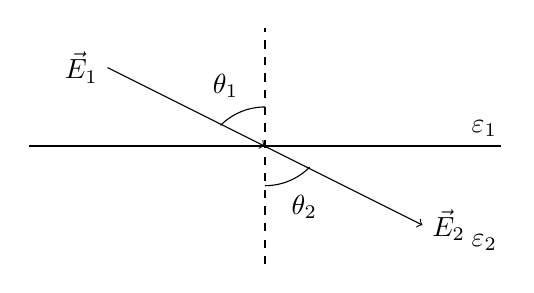
\begin{tikzpicture}
    \draw[thick] (-3,0) -- (3,0);
    \draw[dashed] (0,-1.5) -- (0,1.5);

    % Incident ray
    \draw[->] (-2,1) -- (0,0);
    \node[left] at (-2,1) {$\vec{E}_1$};

    % Reflected ray
    \draw[->] (0,0) -- (2,-1);
    \node[right] at (2,-1) {$\vec{E}_2$};

    % Angle labels
    \draw (0,-0.5) arc (-90:-45:0.8);
    \node[above] at (-0.5,0.5) {$\theta_1$};

    \draw (0,0.5) arc (90:135:0.8);
    \node[below] at (0.5,-0.5) {$\theta_2$};

    % Medium labels
    \node[above right] at (2.5,0) {$\varepsilon_1$};
    \node[below right] at (2.5,-1) {$\varepsilon_2$};
\end{tikzpicture}

\begin{enumerate}
\item $\varepsilon_1\sin{\theta_1}=\varepsilon_2\sin{\theta_2}$
\item $\varepsilon_1\cos{\theta_1}=\varepsilon_2\cos{\theta_2}$
\item $\varepsilon_1\tan{\theta_1}=\varepsilon_2\tan{\theta_2}$
\item $\varepsilon_1\cot{\theta_1}=\varepsilon_2\cot{\theta_2}$
\end{enumerate}

\item If $\vec{E}$ and $\vec{B}$ are the electric and magnetic fields respectively, then $\vec{E}\cdot\vec{B}$ is

\begin{enumerate}
\item odd under parity and even under time reversal
\item even under parity and odd under time reversal
\item odd under parity and odd under time reversal
\item even under parity and even under time reversal
\end{enumerate}

\item A small disc is suspended by a fiber such that it is free to rotate about the fiber axis (see figure). For small angular deflections, the Hamiltonian for the disc is given by $$H=\frac{p^2_\theta}{2I}+\frac{1}{2}\alpha\theta^2$$ where $I$ is the moment of inertia and $\alpha$ is the restoring torque per unit deflection. The disc is subjected to angular deflections ($\theta$) due to thermal collisions from the surrounding gas at temperature $T$ and $p_\theta$ is the momentum conjugate to $\theta$. The average and the root-mean-square angular deflection, $\theta_{avg}$ and $\theta_{rms}$, respectively are

\vspace{0.5 cm}

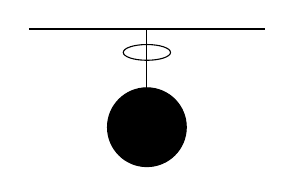
\begin{tikzpicture}
    % Horizontal bar
    \draw[thick] (-1.5,2) -- (1.5,2);

    % Hanging cylinder
    \draw[fill=black] (0,0.75) circle (0.5 cm);
    \draw (0,1.25) -- (0,2);

    % Circular arrow
    \draw[->] (0,1.7) ellipse [x radius=0.3 cm, y radius=0.1 cm, start angle=0, end angle=360];
\end{tikzpicture}

\begin{enumerate}
\item $\theta_{avg}=0$ and $\theta_{rms}=\brak{\frac{k_BT}{\alpha}}^{\frac{3}{2}}$
\item $\theta_{avg}=0$ and $\theta_{rms}=\brak{\frac{k_BT}{\alpha}}^{\frac{1}{2}}$
\item $\theta_{avg}\neq0$ and $\theta_{rms}=\brak{\frac{k_BT}{\alpha}}^{\frac{1}{2}}$
\item $\theta_{avg}\neq0$ and $\theta_{rms}=\brak{\frac{k_BT}{\alpha}}^{\frac{3}{2}}$
\end{enumerate}

\item As shown in the figure, an ideal gas is confined to chamber A of an insulated container, with vacuum in chamber B. When the plug in the wall separating the chambers A and B is removed, the gas fills both the chambers. Which one of the following statements is true?

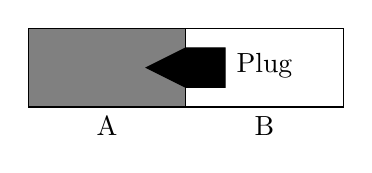
\begin{tikzpicture}
    % Rectangle
    \draw[fill=gray] (-2,0) rectangle (0,1);
    \draw (0,0) rectangle (2,1);

    % Plug
    \draw[fill=black] (-0.5,0.5) -- (0,0.75) -- (0.5,0.75) -- (0.5,0.25) -- (0,0.25) -- cycle;
    \node[above] at (1,0.25) {Plug};

    % Labels
    \node[below] at (-1,0) {A};
    \node[below] at (1,0) {B};
\end{tikzpicture}

\begin{enumerate}
\item The temperature of the gas remains unchanged
\item Internal energy of the gas decreases
\item Temperature of the gas decreases as it expands to fill the space in chamber B
\item Internal energy of the gas increases as its atoms have more space to move around
\end{enumerate}
